\section{Performance evaluation}
\label{section:project_evaluation}

The implementation of Physarum-based Metaheuristic algorithm is tested under variety of conditions. Some tests have been made to show general behaviour of the algorithm depending on input problem size, while other test influence of various parameters, helping out with their selection. In the end the algorithm is compared to other common algorithms.


\subsection{Dataset description}

The algorithm is tested on QAPLIB dataset library \cite{burkard1997qaplib}. This dataset is de~facto standard for testing various Quadratic Assignment Problem solvers. It includes dozens of problem definitions with optimal solutions (or approximations where no optimal solution has been found yet) in unified format. Some of the inputs are synthetic, generated using various algorithms (i.e. \texttt{lipa} or \texttt{nug}), while some problems are taken from the real world (i.e. \texttt{els} or \texttt{ste}).


\subsection{Testing methodology}

Same seed value has been used across the tests, unless mentioned otherwise --- this simple trick ensures the same initial position even if different configuration options are used. Test cases \texttt{lipa20a} and \texttt{lipa90a} are used for testing various parameters as they greatly differ in size ($n=20$ and $n=90$), so influences of the parameters can be observed. Values of observable parameters are measured every epoch (a discrete algorithm step), while execution time is bounded by 300~s limit, unless mentioned otherwise.

All tests have been done on the same test machine with given specification: processor Intel Xeon E3-1246 3.5GHz, DDR3-1600 32GB RAM, Linux kernel 3.19. Every plot used in this work is generated automatically from logs made by \texttt{physarum-debug} (the logs are included with the source). Some detailed numerical values are provided in tables in Appendix \ref{chapter:results}.


\subsection{Colony initialization phase}

The algorithm initialization phase begins with sampling of $k$ random solutions from whole $n!$ search space --- than on $l$ best solution instances of \texttt{Plasmodium} are put. Size of population directly affects total number of visited solutions (solutions that were used as food source when plasmodia crawled), larger populations visit more solutions (figure \ref{figure:am_visited_solutions}), because they start in multiple points of the space search. An obvious observation is that introducing more plasmodia results in more computation, as a result each discrete epoch takes longer time to compute --- these experiments were limited to 300~s execution time, larger colonies finished on earlier epochs.

Larger colonies are merging earlier than smaller colonies (figure \ref{figure:am_state_of_colony}), which is an anticipated behaviour --- the chance of encountering another plasmodium is greater as there are more plasmodia sharing the same space search. It can be observed that as a result of merging number of solutions stops increasing drastically as in early epochs, because there are less plasmodia crawling.

\begin{figure}
  \centering

  \begin{subfigure}{\textwidth}
    \includegraphics[width=1.1\textwidth,center]{algorithm/metaheuristic/charts/single/lipa20a/total_food_eaten_count - lipa20a $l=300$ $k=300$.\eop}
    \caption{instance \texttt{lipa20a} $n=20$}
  \end{subfigure}
  \par\bigskip
  \begin{subfigure}{\textwidth}
    \includegraphics[width=1.1\textwidth,center]{algorithm/metaheuristic/charts/single/lipa90a/total_food_eaten_count - lipa90a $l=300$ $k=300$.zoomed.\eop}
    \caption{instance \texttt{lipa90a} $n=90$}
  \end{subfigure}
  
  \caption{Number of visited solutions with different colony size $l$, samples $k$}
  \label{figure:am_visited_solutions}
\end{figure}

\begin{figure}
  \centering

  \begin{subfigure}{\textwidth}
    \includegraphics[width=1.1\textwidth,center]{algorithm/metaheuristic/charts/single/lipa90a/state of colony - lipa90a $l=10$ $k=30$.\eop}
    \caption{population $l=10$, samples $k=30$}
  \end{subfigure}
  \par\bigskip
  \begin{subfigure}{\textwidth}
    \includegraphics[width=1.1\textwidth,center]{algorithm/metaheuristic/charts/single/lipa90a/state of colony - lipa90a $l=100$ $k=300$.\eop}
    \caption{population $l=100$, samples $k=300$}
  \end{subfigure}
  \par\bigskip
  \begin{subfigure}{\textwidth}
    \includegraphics[width=1.1\textwidth,center]{algorithm/metaheuristic/charts/single/lipa90a/state of colony - lipa90a $l=300$ $k=300$.\eop}
    \caption{population $l=300$, samples $k=300$}
  \end{subfigure}

  \caption{State of colony with different colony size $l$, samples $k$ (instance \texttt{lipa90a} $n=90$)}
  \label{figure:am_state_of_colony}
\end{figure}


\begin{figure}
  \centering

  \begin{subfigure}{\textwidth}
    \includegraphics[width=1.1\textwidth,center]{algorithm/metaheuristic/charts/single/lipa20a/frontier_best_cost aggregated min - lipa20a $l=300$ $k=300$.zoomed.\eop}
    \caption{instance \texttt{lipa20a} $n=20$}
  \end{subfigure}
  \par\bigskip
  \begin{subfigure}{\textwidth}
    \includegraphics[width=1.1\textwidth,center]{algorithm/metaheuristic/charts/single/nug20/frontier_best_cost aggregated min - nug20 $l=300$ $k=300$.zoomed.\eop}
    \caption{instance \texttt{nug20} $n=20$}
  \end{subfigure}
  
  \caption{Cost of the best detected solution by any plasmodium with different colony size $l$, samples $k$}
  \label{figure:am_best_cost}
\end{figure}

For small test cases a regularity has been observed --- larger populations tend to find better results in earlier epochs (figure \ref{figure:am_best_cost}). Furthermore, larger $\frac{l}{k}$ proportions (number of plasmodia vs number of samples) are preferred as they exhibit the same characteristic --- when the same number of samples is used, more plasmodia started on these samples yield better results earlier. Plasmodium initialised on a bad solution can crawl towards better one, where a plasmodium initialised on a relatively good solution may not find any better in its local neighbourhood. Thus one should use $l$ close to $k$ to fully use the algorithm potential. 


\subsection{Energy values}

Essential parts of the algorithm are $E_{explore}$ and $E_{crawl}$ energy values. The first one has direct effect on the size of frontier and number of explored solutions, while the second one has an effect on the size of plasmodium.

Indeed, large values of $E_{explore}$ cause frontier to be rather small, as little solutions can be explored and added as interesting to the frontier (figure \ref{figure:am_energy_frontier}). On the other hand, larger values of $E_{crawl}$ make plasmodium to occupy less food sources (figure \ref{figure:am_energy_size}).

Moreover there is a latent relation between frontier size and $E_{crawl}$ value --- frontier size tend to oscillate when $E_{crawl}$ is rather large (figure \ref{figure:am_energy_frontier}), it is so because a plasmodium must conserve energy for crawl phase instead of exploration phase. We also can notice a strong relationship between $E_{explore}$ and cost of the explored best solution (figure \ref{figure:am_energy_cost}) --- small values of $E_{explore}$ tend to visit minimal solutions in earlier epochs. 

\begin{figure}
  \centering

  \includegraphics[width=1.1\textwidth,center]{algorithm/metaheuristic/charts/energy/frontier aggregated avg - lipa20a $E_{explore}=0.001$ $E_{crawl}=0.001$.zzzoomed.\eop}

  \caption{Average size of frontier for colonies with different energies $E_{explore}$ and $E_{crawl}$ (dataset \texttt{lipa20a} $n=20$, $l=10$, $k=30$)}
  \label{figure:am_energy_frontier}
\end{figure}

\begin{figure}
  \centering

  \includegraphics[width=1.1\textwidth,center]{algorithm/metaheuristic/charts/energy/size aggregated avg - lipa20a $E_{explore}=0.001$ $E_{crawl}=0.001$.zzzoomed.\eop}

  \caption{Average size of plasmodia for colonies with different energies $E_{explore}$ and $E_{crawl}$ (dataset \texttt{lipa20a} $n=20$, $l=10$, $k=30$)}
  \label{figure:am_energy_size}
\end{figure}

\begin{figure}
  \centering

  \includegraphics[width=1.1\textwidth,center]{algorithm/metaheuristic/charts/energy/frontier_best_cost aggregated min - lipa20a $E_{explore}=0.001$ $E_{crawl}=0.001$.zzzoomed.\eop}

  \caption{Cost of the best detected solution by any plasmodium with different energies $E_{explore}$ and $E_{crawl}$ (dataset \texttt{lipa20a} $n=20$, $l=10$, $k=30$)}
  \label{figure:am_energy_cost}
\end{figure}

Another parameter that can be used to tune the algorithm is $E_{initial}$ --- initial quanta of energy given to plasmodia on their initialization. Experiments have shown that it has little to none meaning in usual cases. A clear change is visible in frontier size at the first epoch (figure \ref{figure:am_energy_initial}) --- with bigger $E_{initial}$ there is more energy so more exploration steps can be done (each using $E_{explore}$). In tested cases it has little effect on the solution, however one can imagine a large instance of QAP where thorough exploration of neighbours on initialization can in fact result in finding close to optimal solution at early stages.

\begin{figure}
  \centering

  \includegraphics[width=1.1\textwidth,center]{algorithm/metaheuristic/charts/initial90/frontier aggregated avg - lipa90a $E_{initial}=10.0$.zzzoomed.\eop}

  \caption{Average frontier size with different initial energy $E_{initial}$ (dataset \texttt{lipa90a} $n=90$, $l=10$, $k=30$)}
  \label{figure:am_energy_initial}
\end{figure}

An unfortunate consequence of the algorithm design is $O(n!)$ space complexity (figure \ref{figure:am_energy_spacetime}). If every solution is visited, ${\Delta}E_{solution}$ values  must be stored $n!$ times, however this is the worst case scenario, rather not likely to happen in practice. Rather small number of solutions are crawled and occupied during work of the program, it would require extremely small $E_{explore}$ values to force algorithm to occupy every solution, therefore using $O(n!)$ memory and $O(n!)$ computation steps - using sane values of energy averts these adverse effects. As more solutions are explored, lower number of epochs is done, as whole computation time is given to exploration phase.

\begin{figure}
  \centering

  \begin{subfigure}{\textwidth}
    \includegraphics[width=1.1\textwidth,center]{algorithm/metaheuristic/charts/energy/memory - lipa20a $E_{explore}=0.001$ $E_{crawl}=0.001$.\eop}
    \caption{Memory usage}
  \end{subfigure}
  \par\bigskip
  \begin{subfigure}{\textwidth}
    \includegraphics[width=1.1\textwidth,center]{algorithm/metaheuristic/charts/energy/time - lipa20a $E_{explore}=0.001$ $E_{crawl}=0.001$.\eop}
    \caption{Total time}
  \end{subfigure}
  
  \caption{Resources usage with different $E_{explore}$ and $E_{crawl}$ (dataset \texttt{lipa20})}
  \label{figure:am_energy_spacetime}
\end{figure}


\subsubsection{Random walk}

Some combinations of $E_{explore}$ and $E_{crawl}$ can result in meaningless "random walk" and should be avoided. When $E_{explore}$ and $E_{crawl}$ are of similar value and their sum is close to unit value (energy of best solution from the sampling phase), plasmodia will choose any solution no matter their energetic value and corresponding cost (figure \ref{figure:am_energy_random}). Such behaviour omits any optimization behaviour, crawling to solutions without any benefits, hence the name random walk.

\begin{figure}
  \centering

  \includegraphics[width=1.1\textwidth,center]{algorithm/metaheuristic/charts/random/frontier_best_cost for each plasmodium - random $E_{crawl}=0.001$ $E_{explore}=0.5$.\eop}

  \caption{Cost of best solution in frontier for every plasmodium with random walk conditions $E_{crawl}=0.3$, $E_{explore}=0.5$ (dataset \texttt{lipa20a} $n=20$, $l=10$, $k=30$)}
  \label{figure:am_energy_random}
\end{figure}

\subsubsection{Plasmodial death}
% TODO plasmodial death

Extreme values of $E_{explore}$ combined with large values $E_{crawl}$ results in premature plasmodium death. Instead of merging or lasting until the time limit, multiple plasmodia die as they lack energy for crawling to another solution and gaining some new energy (figure \ref{figure:am_energy_death}).

\begin{figure}
  \centering

  \begin{subfigure}{\textwidth}
    \includegraphics[width=1.1\textwidth,center]{algorithm/metaheuristic/charts/death/state of colony - lipa20a $E_{crawl}=0.49$ $E_{explore}=0.5$.\eop}
    \caption{$E_{explore}=0.5$, $E_{crawl}=0.49$}
  \end{subfigure}
  \par\bigskip
  \begin{subfigure}{\textwidth}
    \includegraphics[width=1.1\textwidth,center]{algorithm/metaheuristic/charts/death/state of colony - lipa20a $E_{crawl}=0.45$ $E_{explore}=0.5$.\eop}
    \caption{$E_{explore}=0.5$, $E_{crawl}=0.45$}
  \end{subfigure}
  
  \caption{State of colony with different extreme $E_{explore}$ and $E_{crawl}$ (dataset \texttt{lipa20a} $n=20$, $l=10$, $k=30$)}
  \label{figure:am_energy_death}
\end{figure}


\subsection{Cost to food transformation}

An important step is the cost to food transformation --- each solution's cost is transformed into nutritional energy using equation \ref{equation:m_e_solution}. Every solution is compared to the best solution from the sampling phase, every quotient $\frac{calibrated\_cost}{cost(solution)}$ is amplified using exponential function with exponential function with the  base $q$, linearly scaled using coefficient $a$ (usually $a=q^{-1}$). 

Using such transformation gives solutions equal to the best sample an unit value of $E_{solution}=1$, worse solutions carry lower energy, while better solutions carry bigger energy. Modifying the base $q$ (and corresponding scale $a$) can be used to intensify this difference.

\begin{figure}
  \centering

  \includegraphics[width=1.1\textwidth,center]{algorithm/metaheuristic/charts/ctf/food aggregated sum - lipa20a $a=0.25$ $q=4$.zoomed.\eop}
  
  \caption{Plasmodium energy $E_{plasmodium}$ with different base $q$ and scale $a$ (dataset \texttt{lipa20a} $n=20$, $l=1$, $k=10$)}
  \label{figure:am_ctf_food}
\end{figure}

\begin{figure}
  \centering

  \includegraphics[width=1.1\textwidth,center]{algorithm/metaheuristic/charts/ctf/frontier aggregated min - lipa20a $a=0.25$ $q=4$.zoomed.\eop}
  
  \caption{Size of frontier with different base $q$ and scale $a$ (dataset \texttt{lipa20a} $n=20$, $l=1$, $k=10$)}
  \label{figure:am_ctf_frontier}
\end{figure}

Experiments confirm that larger $q$ values provide more energy to plasmodia (figure \ref{figure:am_ctf_food}) as explored solution carry more $E_{solution}$ energy. This extra energy is used for exploration phase and result in larger frontier sizes (figure \ref{figure:am_ctf_frontier}).


\subsection{Optimization results}

In order to assess usefulness of the Physarum-based Metaheuristic algorithm two measures are used: relative distance to optimal solution and assignment similarity measure. The relative distance is defined as follows:
\begin{equation}
  dist(cost, optimum) = \frac{cost - optimum}{optimum}
\end{equation}
Where $cost$ is the cost of compared solution and $optimum$ is optimum (or its best known approximation) given as input data from \texttt{QAPLIB}. With such measure values closer to $0.0$ are preferred, as they are closer to the optimal cost.

The similarity measure aggregated differences in the assignment to simple real value. The similarity is defined as fraction of assignments on the same position:
\begin{equation}
  sim(a, b) = \frac{| x : a(x) = b(x), x \in [1, n] \subset \mathbb{N}|}{|n|}
\end{equation}
Where $a$ and $b$ are compared assignment and $n$ is the problem size. This measure is defined between zero and one, with $sim(a, b) = 0$ meaning complete mismatch and $sim(a, b) = 1$ meaning complete match. One should notice that an assignment can be optimal ($dist=0$), even though its $sim(a, opt) \leq 1$ --- multiple assignments can yield the same optimal cost.

The first experiments have been done on \texttt{lipa} dataset, which is made of 8 different problem definitions of size $n \in {20, 30, 40, 50, 60, 70, 80, 90}$. An universal values of $E_{explore}=0.001$ and $E_{crawl}=0.01$, scaling factor $a=0.1$, exponential base $q=10$, population size $l=100$ out of $k=300$ samples, time of execution was made relative to input size $t=4n$.

\begin{figure}
  \centering

  \begin{subfigure}{0.47\textwidth}
    \includegraphics[width=1.0\textwidth]{algorithm/metaheuristic/charts/complipaoriginal/distance.eps}
    \caption{Distance to the optimal solution}
  \end{subfigure}
  \begin{subfigure}{0.47\textwidth}
    \includegraphics[width=1.0\textwidth]{algorithm/metaheuristic/charts/complipaoriginal/similarity.eps}
    \caption{Similarity with optimal assignment}
  \end{subfigure}
  
  \caption{Results for \texttt{lipa} dataset}
  \label{figure:am_lipa_results}
\end{figure}

Obtained results (figure \ref{figure:am_lipa_results}) look promising, but are not truly satisfactory. For small instances relative error is quite large, even though most of the assignment is the same as the optimal assignment. A conclusion can be made, that plasmodium is close to the solution, however it might have missed it or crawled out of it. Furthermore, for larger instances almost there is almost no similarity between computed and optimal assignment, even though relative distance is acceptable ($dist < 1\%$) --- the plasmodia have crawled into local minima, far from optimal neighbourhood.

\subsubsection{Improved algorithm}

A solution for this sub-efficient behaviour has been quickly found. In earlier evaluations of the algorithm (figure \ref{figure:am_best_cost}), we observed that plasmodia can crawl out of optimal solutions. This behaviour is a result of plasmodia avoiding being stuck in a local optimum, however it has no knowledge if the optimum is local or a global minimum. 

At this point a minor improvement to the algorithm has been added --- each plasmodium stores the best solution it explored during its lifetime. This does not change a behaviour of the plasmodium, it just adds another observation of plasmodial behaviour. While original algorithm returned the best occupied solution by any plasmodium, the improved algorithm returns the best solution ever found by any plasmodium.

\begin{figure}
  \centering

  \begin{subfigure}{0.9\textwidth}
    \includegraphics[width=1.0\textwidth]{algorithm/metaheuristic/charts/complipaimproved/distance.eps}
    \caption{Distance to the optimal solution}
  \end{subfigure}
  \begin{subfigure}{0.9\textwidth}
    \includegraphics[width=1.0\textwidth]{algorithm/metaheuristic/charts/complipaimproved/similarity.eps}
    \caption{Similarity with optimal assignment}
  \end{subfigure}
  
  \caption{Results for \texttt{lipa} dataset for original and improved algorithm}
  \label{figure:am_lipa_results_improved}
\end{figure}

As predicted this change made a positive influence on the results (figure \ref{figure:am_lipa_results_improved}). For \texttt{lipa20a} and \texttt{lipa30a} optimal assignment have been found, where for other instances of \texttt{lipa}, assignments worse only less than $1~\%$ from the optimum have been found. Furthermore the improved implementation has been tested with longer execution time $t=10n$ instead $t=4n$, which has given slightly better results The improved version of algorithm provides better result and it will be used for further tests.


\subsubsection{QAPLIB results}

Using generic parameters (population $l=100$, samples $k=300$, $E_{explore}=0.001$, $E_{crawl}=0.01$, exponential base $q=10$ scale $a=0.1$), tests for every case in \texttt{QAPLIB} have been done. Every test has been repeated ten times, no random seed has been preset as in practical usage. Results are aggregated in different ways --- by minimum cost (showing the best case) and by average cost presenting an usual result for given dataset. Every instance has been allowed to run for time $t=10n$, but no longer than 900~s.


\newcommand{\qaplibresultchart}[1]{
  \begin{figure}
    \centering

    \begin{subfigure}{0.47\textwidth}
      \includegraphics[width=1.0\textwidth]{algorithm/metaheuristic/charts/multiple/#1/distance.eps}
      \caption{Distance to the optimal solution}
    \end{subfigure}
    \begin{subfigure}{0.47\textwidth}
      \includegraphics[width=1.0\textwidth]{algorithm/metaheuristic/charts/multiple/#1/similarity.eps}
      \caption{Similarity with optimal assignment}
    \end{subfigure}
    
    \caption{Aggregated results for \texttt{#1} dataset}
    \label{figure:am_qaplib_result:#1}
  \end{figure}
}

\qaplibresultchart{bur}
\qaplibresultchart{chr}
\qaplibresultchart{had}
\qaplibresultchart{lipaa}
\qaplibresultchart{lipab}
\qaplibresultchart{nug}
\qaplibresultchart{rou}
\qaplibresultchart{scr}
\qaplibresultchart{sko}
\qaplibresultchart{tai}

% TODO complete run for qaplib
% TODO some charts grouped by dataset

% TODO table in appendix b (optimal solution, each case, avg, stderr, similarity and cost for best)

\subsubsection{Optimising large instances}

% TODO some parameters

\subsection{Final results}
% TODO comparison with other - wiola, juskowiak&pewinski
% TODO table in appendix b (our solution vs other solutions)
